\subsection{NATaS : ordonnancer des tâches sur une machine NUMA}
Ne trouvant pas de solution adaptée à notre besoin, nous avons créer notre propre ordonnanceur de tâches.
%
Nous l'avons appelé NATaS, il s'agit de l'acronyme {\em Numa Aware Task Scheduler}.
%
Celui-ci est très basique, il ne prend en compte que l'affinité mémoire des tâches, la gestion des dépendances est laissée à Taggre, tout comme avec les ordonnanceurs OpenMP et TBB.
%
Pour ordonnancer les tâches avec la meilleurs affinité mémoire possible, nous utilisons un conteneur de tâches thread-safe par banc NUMA.
%
Ce container permet à plusieurs threads d'insérer/retirer des tâches en limitant la contention.
%
Le vol de tâche entre conteneur a aussi été implémenter, il existe une option par tâche pour autoriser ou non le vol de tâche.
%
Dans le cas du parallélisme de boucle, une option permettant de donner une tâche spécifiquement à un thread a été implémentée.


Contrairement à la plupart des autres ordonnanceurs de tâches, nous n'utilisons pas un conteneur de tâches par thread mais un conteneur par banc NUMA.
%
Nous avons donc plus de contention sur cette structure et une queue basique ne serai pas assez efficace.
%
\`A la place, nous utilisons un conteneur sans verrou, entièrement construit autour de l'instruction compare-and-swap.
%

%
Cette structure ne nous permet pas d'obtenir les mêmes performances que l'utilisation d'une queue par thread, mais elle a l'avantage de mieux fonctionner pour l'équilibrage de charge à l'intérieur d'un banc NUMA.



NATaS fourni aussi une api permettant de gérer les allocations mémoires et leurs placements.
%
Il permet de faire différents types d'allocations tel que :
\begin{itemize}
  \item distribuer régulièrement la mémoire;
  \item entrelacer les pages mémoires;
  \item spécifier l'emplacement mémoire.
\end{itemize}
%
Ces allocations font miroir au différent type d'ordonnancements (first touch, interleave and bind).
%
Dans le cas d'un parallélisme de boucle avec un distribution statique, on distribuera la mémoire régulièrement.
%
Dans le cas d'un graphe de tâche, le programmeur donnera la position souhaitée des tâches.
%
Pour cela, il lui suffira de simuler l'exécution du code, de désactiver le vol de tâches et d'appeler la fonction d'allocation ou de migration des pages dans chaque tâche.
%
Nous obtiendrons ainsi une mémoire équitablement distribuée et des accès mémoire optimisés.


NATaS s'interface avec Taggre pour améliorer les performances sur des machines NUMA.
%
La connaissance complète du graphe de tâche permet des améliorations notables sur la distribution mémoire.
%
Comme le graphe sera déroulé de haut en bas lors de son exécution, il parait naturel de distribuer les tâches par hauteur.
%
En supposant que les tâches produisent des données et que ces données sont passées en paramètre aux tâches successeurs dans le graphe, on peut essayer d'optimiser le placement NUMA.
%
Dans un premier temps, on va équilibrer la distribution des tâches sur les bancs NUMA en attribuant une affinité NUMA aux tâches.
%
Cette affinité sera choisie en fonction de la hauteur de la tâche dans le graphe et des affinités NUMA de ses prédécesseurs.
%
Le but étant d'avoir à hauteur fixée, un nombre égale de tâche par banc NUMA tout en minimisant les accès en lecture distant.



%   (-_-)   %
\begin{figure}[t!]
  \centering
  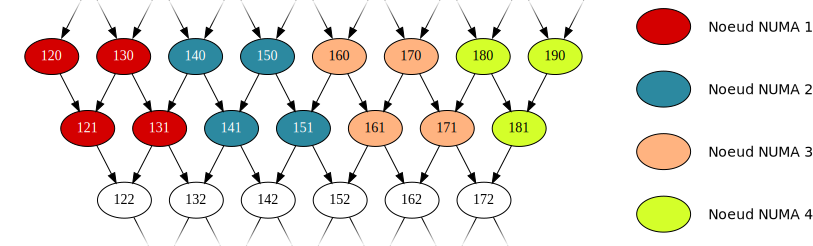
\includegraphics[width=\textwidth]{numa_distrib_example}
  \caption{Exemple de l'algorithme de distribution des tâches en action, la couleur des tâches détermine leurs affinités NUMA. Les tâches en blanches ne sont pas encore traitées.}
  \label{fig:numa_distrib_example}
\end{figure}
